\chapter{O Campo Elétrico}

\begin{lstlisting}[language=Python, frame=lines,basicstyle=\footnotesize, caption={Linhas de campo de um multipolo.}, label={lst:Multipole}]
import numpy as np
import matplotlib.pyplot as plt
from matplotlib.patches import Circle

def E(q, r0, x, y):
    """Return the electric field vector E=(Ex,Ey) due to charge q at r0."""
    den = np.hypot(x-r0[0], y-r0[1])**3
    return q * (x - r0[0]) / den, q * (y - r0[1]) / den

# Grid of x, y points
nx, ny = 64, 64
x = np.linspace(-2, 2, nx)
y = np.linspace(-2, 2, ny)
X, Y = np.meshgrid(x, y)

# Create a multipole with nq charges of alternating sign, equally spaced
# on the unit circle.
nq = 10
charges = []
for i in range(nq):
    q = i%2 * 2 - 1
    charges.append((q, (np.cos(2*np.pi*i/nq), np.sin(2*np.pi*i/nq))))

# Electric field vector, E=(Ex, Ey), as separate components
Ex, Ey = np.zeros((ny, nx)), np.zeros((ny, nx))
for charge in charges:
    ex, ey = E(*charge, x=X, y=Y)
    Ex += ex
    Ey += ey

fig = plt.figure(figsize=(10, 10), dpi=100)
ax = fig.add_subplot(111)

# Plot the streamlines with an appropriate colormap and arrow style
color = 2 * np.log(np.hypot(Ex, Ey))
ax.streamplot(x, y, Ex, Ey, color=color, linewidth=1, cmap=plt.cm.inferno,
              density=2, arrowstyle='->', arrowsize=1.5)

# Add filled circles for the charges themselves
charge_colors = {True: '#aa0000', False: '#0000aa'}
for q, pos in charges:
    ax.add_artist(Circle(pos, 0.05, color=charge_colors[q>0]))

ax.set_xlabel('$x$')
ax.set_ylabel('$y$')
ax.set_xlim(-2,2)
ax.set_ylim(-2,2)
ax.set_aspect('equal')
plt.show()
\end{lstlisting}

\begin{figure}[h!]
\centering
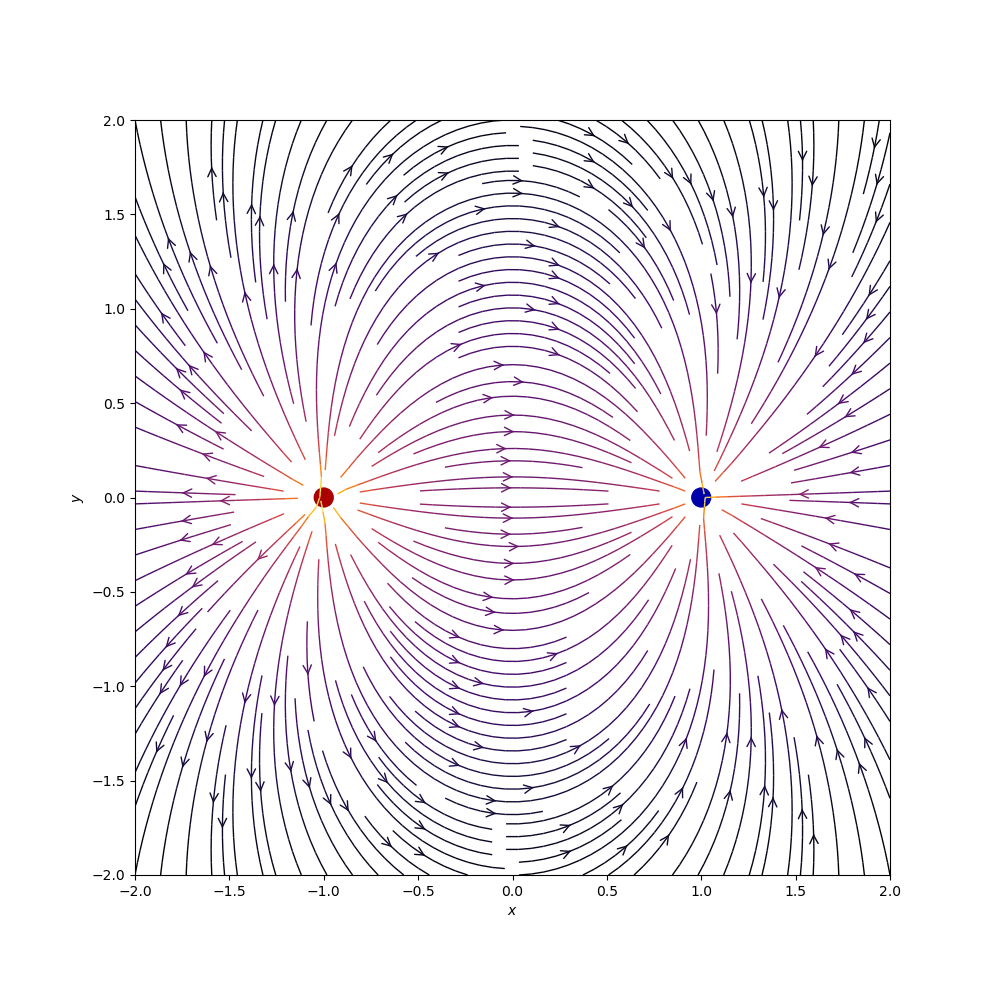
\includegraphics[scale=0.6]{Images/dipolo.png}
\caption{Linhas de Campo em um capacitor de um dipolo}\label{fig:dipole-saida}
\end{figure}

\begin{lstlisting}[language=Python, frame=lines,basicstyle=\footnotesize, caption={Linhas de campo de um capacitor de placas paralelas.}, label={lst:Capacitor}]
import numpy as np
import matplotlib.pyplot as plt
from matplotlib.patches import Circle

WIDTH, HEIGHT, DPI = 700, 700, 100

def E(q, r0, x, y):
    """Return the electric field vector E=(Ex,Ey) due to charge q at r0."""
    den = ((x-r0[0])**2 + (y-r0[1])**2)**1.5
    return q * (x - r0[0]) / den, q * (y - r0[1]) / den

# Grid of x, y points
nx, ny = 128, 128
x = np.linspace(-5, 5, nx)
y = np.linspace(-5, 5, ny)
X, Y = np.meshgrid(x, y)

# Create a capacitor, represented by two rows of nq opposite charges separated
# by distance d. If d is very small (e.g. 0.1), this looks like a polarized
# disc.
nq, d = 20, 2
charges = []
for i in range(nq):
    charges.append((1, (i/(nq-1)*2-1, -d/2)))
    charges.append((-1, (i/(nq-1)*2-1, d/2)))

# Electric field vector, E=(Ex, Ey), as separate components
Ex, Ey = np.zeros((ny, nx)), np.zeros((ny, nx))
for charge in charges:
    ex, ey = E(*charge, x=X, y=Y)
    Ex += ex
    Ey += ey

fig = plt.figure(figsize=(WIDTH/DPI, HEIGHT/DPI), facecolor='w')
ax = fig.add_subplot(facecolor='w')
fig.subplots_adjust(left=0, right=1, bottom=0, top=1)

# Plot the streamlines with an appropriate colormap and arrow style
color = np.log(np.sqrt(Ex**2 + Ey**2))
ax.streamplot(x, y, Ex, Ey, color=color, linewidth=1, cmap=plt.cm.plasma,
              density=3, arrowstyle='->')

# Add filled circles for the charges themselves
charge_colors = {True: '#aa0000', False: '#0000aa'}
for q, pos in charges:
    ax.add_artist(Circle(pos, 0.05, color=charge_colors[q>0], zorder=10))

ax.set_xlabel('$x$')
ax.set_ylabel('$y$')
ax.set_xlim(-5,5)
ax.set_ylim(-5,5)
ax.set_aspect('equal')
plt.savefig('capacitor.png', dpi=DPI)
plt.show()
\end{lstlisting}

\begin{figure}[h!]
\centering
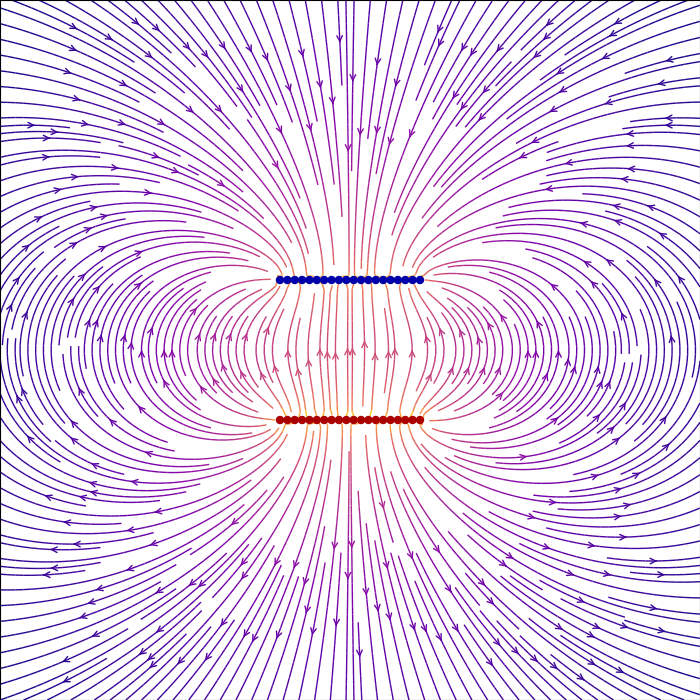
\includegraphics[scale=0.6]{Images/capacitor.png}
\caption{Linhas de Campo em um capacitor de placas paralelas}\label{fig:capacitor-saida}
\end{figure}

Problemas do Haliday Capítulo 21 a 25

Calcule a força de atração entre dois anéis com cargas uniformemente distribuídas $+q$ e $-q$. O eixo dos anéis coincide com o eixo $x$ e cada anel tem raio $R$.

Problema Repetir para um disco e para uma esfera

Um anel de raio $R = 1 cm$ esta uniformemente carregado com carga $Q$. Um elétron se move no plano do anel. (a) Com  $Q= -100 \mu C$ Encontre a velocidade do elétron para que ele se mova  em u